\documentclass[crop=false, class=book]{standalone}

%impostazioni lingua
\usepackage[T1]{fontenc}
\usepackage[utf8]{inputenc}
\usepackage[english,italian]{babel}

%sistema i margini
\usepackage{geometry}
\geometry{a4paper,top=2.2cm,bottom=2.2cm,left=3cm,right=3cm, heightrounded}

%interlinea 1.5
\usepackage{setspace}
\onehalfspacing

%gestione delle testatine
\usepackage{fancyhdr}
\pagestyle{fancy}
\lhead{}
\chead{}
\rhead{Titolo}
\lfoot{}
\cfoot{\thepage}
\rfoot{}
\renewcommand{\headrulewidth}{0.4pt}

%formattazione titoli paragrafo
\usepackage{titlesec}
\titleformat{\chapter}[block]{\normalfont\huge\bfseries}{\thechapter.}{0.7em}{\huge}

%pacchetti per i riferimenti in bibliografia
\usepackage[autostyle,italian=guillemets]{csquotes}
\usepackage[style=numeric,citestyle=numeric-comp,backend=biber]{biblatex}

%risorsa che contiene la bibliografia
\addbibresource{./bibliografia.bib}

%pacchetto per immagini
\usepackage{graphicx}
\usepackage{subfig}

\usepackage[italian]{varioref}
\usepackage{copyrightbox}
\usepackage{url}


\usepackage{lipsum}

\begin{document}
	\chapter{Augmented faces}
	L'API \textit{Augmented Faces} permette di identificare i volti umani e le varie parti che lo compongono tramite Intelligenza Artificiale, per sovrapporre ad essi modelli 3D come maschere, occhiali, cappelli utilizzando solo la fotocamera frontale \cite{google2022faces}. 
	Questa libreria permette ottenere un \textit{face mesh}, una rappresentazione virtuale composta da una maglia di punti che riproduce il profilo del volto \cite{oufqir2020arkit}. Oltre ad essa, l'API fornisce un \textit{center pose} e tre \textit{region pose}, come descritti dalla figura~\vref{fig:augm_faces}.
	
	\paragraph*{Face mesh}
		Consiste in una rete di 468 punti, che permette di posizionare una texture sul volto. Essa viene tracciata come un piano, per permettere all'immagine virtuale di seguire il volto anche se in movimento, come spiegato in \cite{googleblog2019faces}.
	
	\paragraph*{Center pose}
		Rappresenta il centro del volto, posizionato dietro il naso. Utile per il rendering di oggetti virtuali da posizionare sopra la testa.
	
	\paragraph*{Region pose}
		Identifica una regione rilevante del volto, come i lati destro o sinistro della fronte, oppure il naso. Sono utili per il rendering di oggetti virtuali da posizionare sul naso o attorno agli orecchi.
	
	\begin{figure}
		\centering
		\copyrightbox[b]{
			\subfloat[][\emph{Esempio di face mesh}]
			{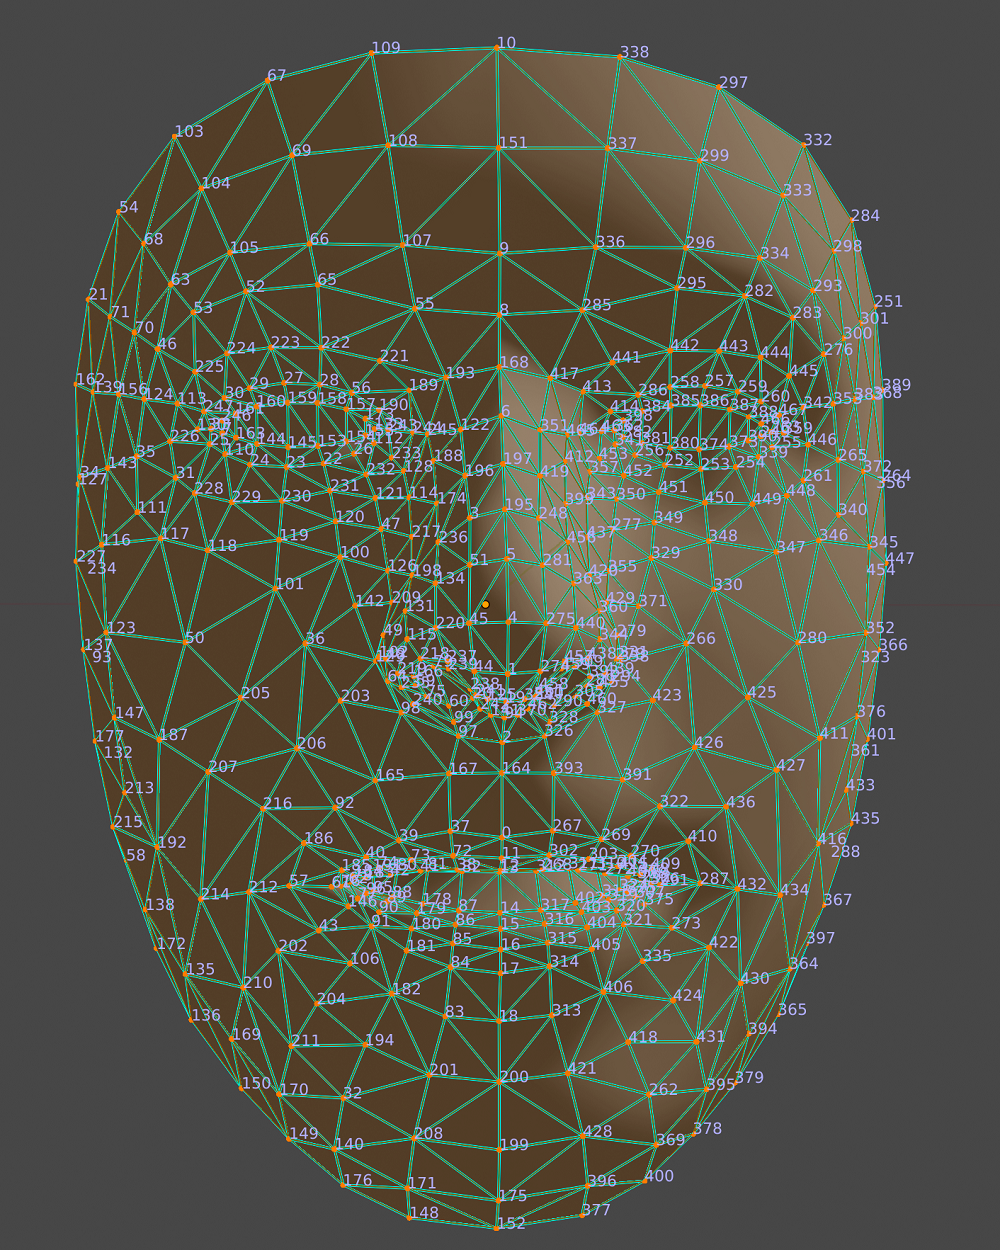
\includegraphics[width=0.31\textwidth]{./resources/images/face_mesh}}  \,
			\subfloat[][\emph{Posizione del center pose}]
			{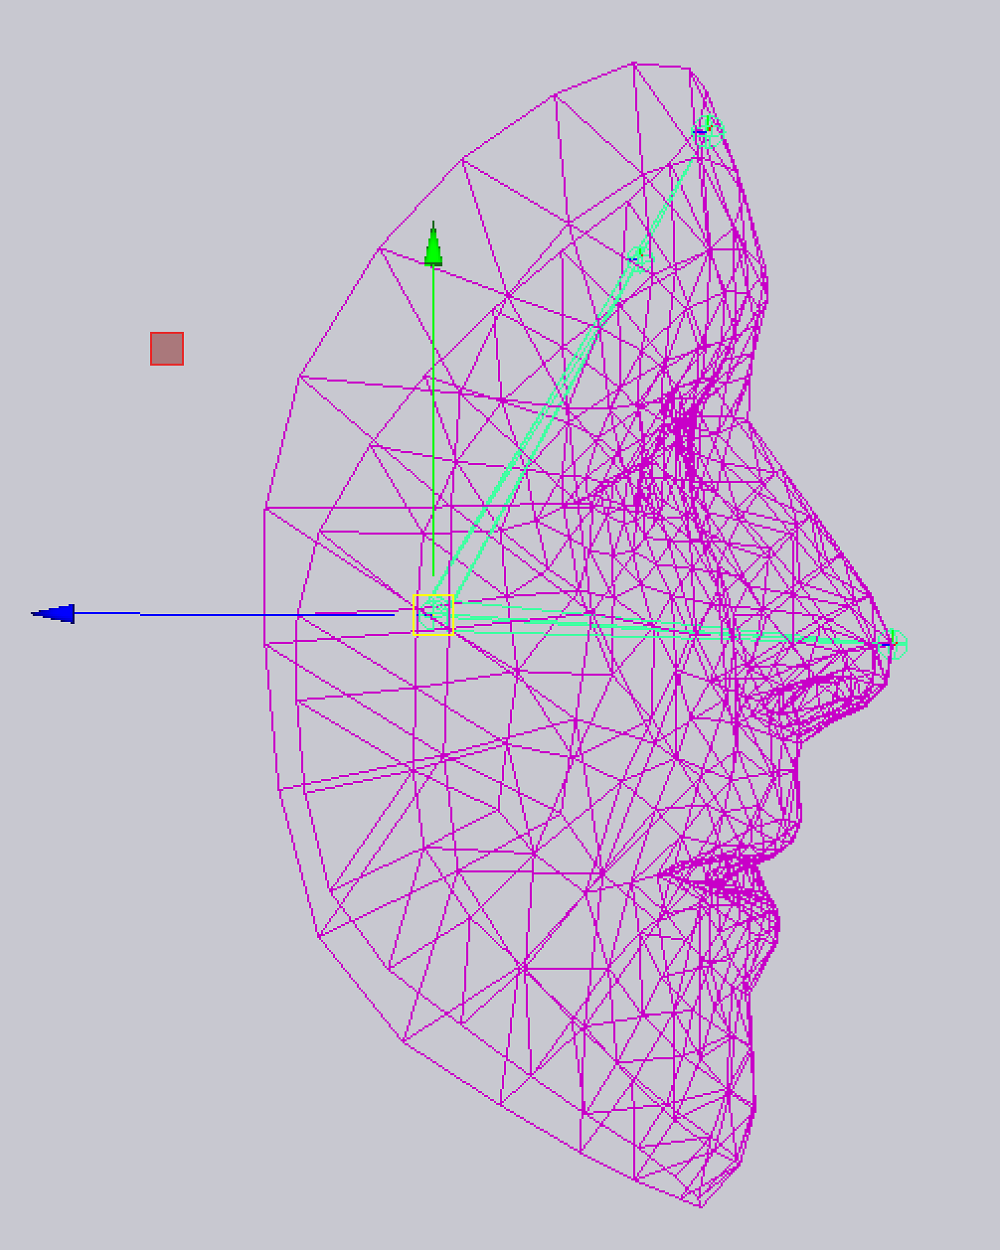
\includegraphics[width=0.31\textwidth]{./resources/images/center_pose}} \,
			\subfloat[][\emph{Posizioni di tre region pose}]
			{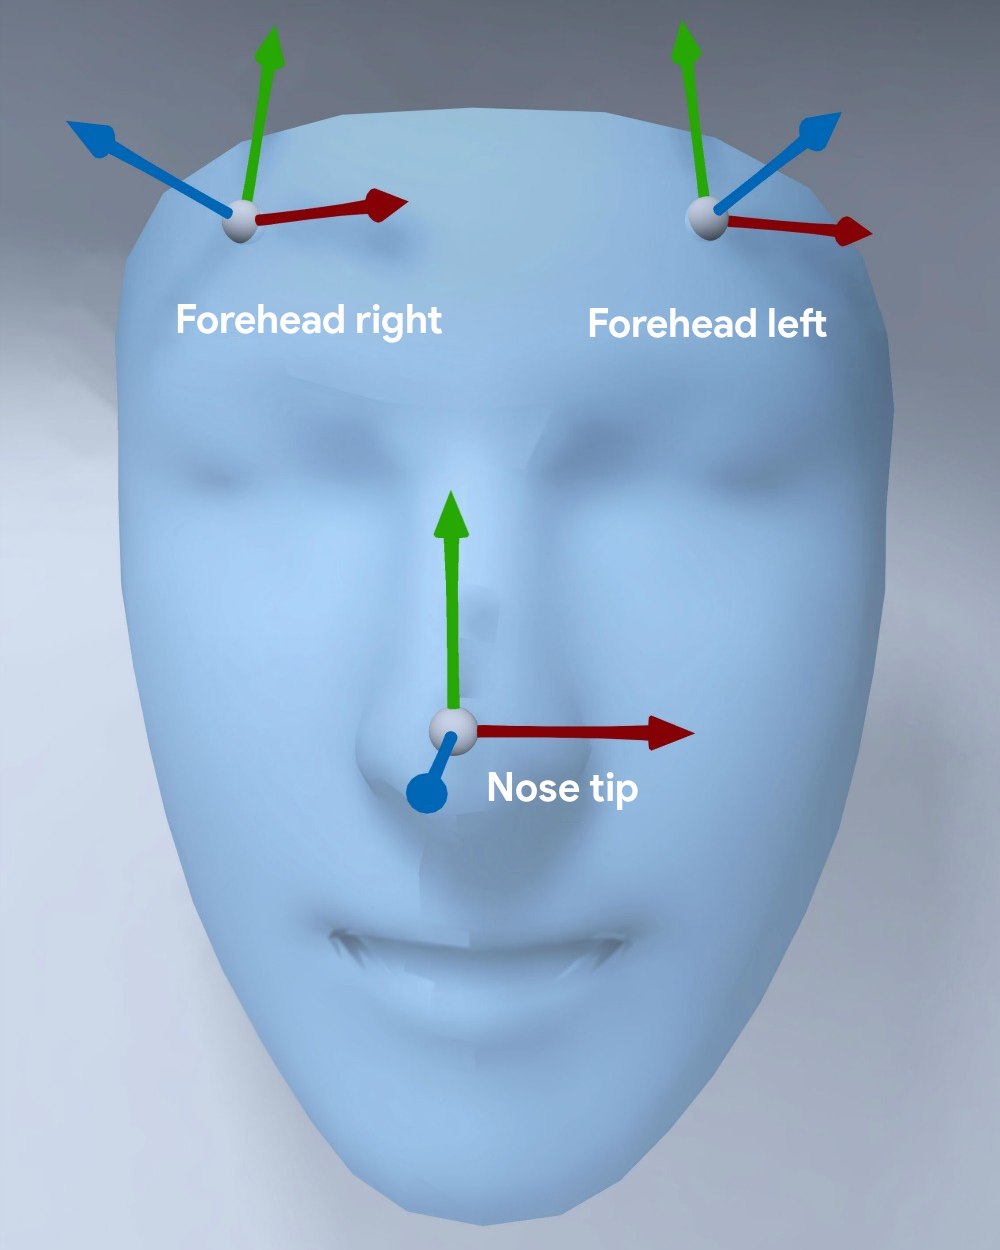
\includegraphics[width=0.31\textwidth]{./resources/images/region_poses}}
		}{Fonte: \url{https://developers.google.com/}}	
		\caption{Elementi ottenuti tramite l'API Augmented Faces}
		\label{fig:augm_faces}
	\end{figure}
	
	\paragraph*{}
	La configurazione della sessione ARCore deve essere effettuata selezionando la fotocamera frontale ed abilitando la modalità Augmented Face, come mostrato nel listing~\vref{lst:af_session} tratto dalla guida ufficiale Google.

	\begin{center}
		\begin{minipage}{0.95\textwidth}
			\begin{lstlisting}[caption={Configurazione della modalità Augmented Face.}, label={lst:af_session}, language=Kotlin]
			// Configura la sessione utilizzando la camera frontale.
			val filter = CameraConfigFilter(session).setFacingDirection(CameraConfig.FacingDirection.FRONT)
			val cameraConfig = session.getSupportedCameraConfigs(filter)[0]
			session.cameraConfig = cameraConfig
			
			// Abilita la modalità Augmented Face.
			val config = Config(session)
			config.augmentedFaceMode = Config.AugmentedFaceMode.MESH3D
			session.configure(config)
			\end{lstlisting}
		\end{minipage}
	\end{center}
	Da ogni frame è possibile ricavare un oggetto \verb|Trackable|, che può essere tracciato e a cui possono essere collegate degli \verb|Anchor|. Verificando lo stato di ogni oggetto \verb|Trackable| restituito, è possibile ricavare i region pose, il center pose e i vertici del face mesh, per poi procedere con il rendering degli oggetti virtuali. Si veda il listing~\vref{lst:faces_use} tratto dalla documentazione ufficiale per un possibile utilizzo.
	
	\begin{center}
		\begin{minipage}{0.95\textwidth}
			\begin{lstlisting}[caption={Utilizzo della modalità Augmented Faces.}, label={lst:faces_use}, language=Kotlin]
			// Ricava gli oggetti trackable dalla sessione ARCore
			val faces = session.getAllTrackables(AugmentedFace::class.java)
			
			// Verifica lo stato di ogni oggetto contenuto nella lista di Trackable
			faces.forEach { face ->
				if (face.trackingState == TrackingState.TRACKING) {
					// Ricava il center pose
					val facePose = face.centerPose
					
					// Ricava i region pose
					val forheadLeft = face.regionPose(AugmentedFace.RegionType.FOREHEAD_LEFT)
					val forheadRight=face.regionPose(AugmentedFace.RegionType.FOREHEAD_RIGHT)
					val noseTip = face.regionPose(AugmentedFace.RegionType.NOSE_TIP)
					
					// Ricava i vertici del face mesh
					val faceVertices = face.meshVertices
					
					// Rendering dell'oggetto virtuale
					// ...
				}
			}
			\end{lstlisting}
		\end{minipage}
	\end{center}
	


	
	
\end{document}